\documentclass[UTF-8]{ctexart}


\usepackage{booktabs}
\usepackage{url}
\usepackage{cite}
\usepackage[version=4]{mhchem}
\usepackage{graphicx}
\usepackage{subfigure}
\usepackage[a4paper,top=2cm,bottom=2cm,right=3cm,left=3cm,marginparwidth=1.75cm]{geometry}
\usepackage{amsmath}
\usepackage{overpic} 
\usepackage{upgreek}

\title{Dot Blot 实验报告}
\author{闫皓铭\\ 2300017744}
\date{2025年2月21日}


\begin{document}
\maketitle
\section{实验目的}
本实验旨在通过Dot Blot技术,利用BP探针(BP Probe)和BA探针(BA Probe)对RNA进行标记,并比较其效果。
通过使用这两种不同的探针,评估其在标记RNA分子中的灵敏度以及与空白对照组的差异。
通过实验,我们将可以了解BP探针和BA探针在RNA标记中的应用表现。
\section{实验原理}
\subsection{APEX2酶标记RNA}
利用APEX2催化过氧化氢\ce{H2O2}与探针(Biotin-phenol and Biotin-aniline)反应,生成高度反应性的自由基,这些自由基可以与周围的RNA分子进行共价结合。
两种探针的结构式如图\ref{探针结构}所示\cite{paper}。
 % Figure
 \begin{figure}[h]
    \centering
    \subfigure[产生自由基的官能团]{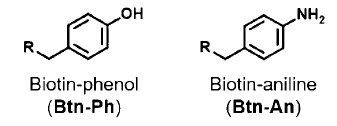
\includegraphics[width=0.4\linewidth]{../Figures/probe structure1.jpg}}
    \subfigure[Biotin]{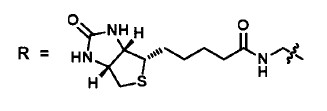
\includegraphics[width=0.4\linewidth]{../Figures/probe structure2.jpg}}
    \caption{探针结构\cite{paper}}  
    \label{探针结构}
 \end{figure}

 后续的显色过程借助了SA-HRP蛋白。这是Streptavidin与Horseradish Peroxidase的融合蛋白,前者负责与Biotin特异性结合,也就是和目标RNA特异性结合,后者用于催化发光液显色\cite{HP}。

 \begin{figure}
    \centering
    \subfigure{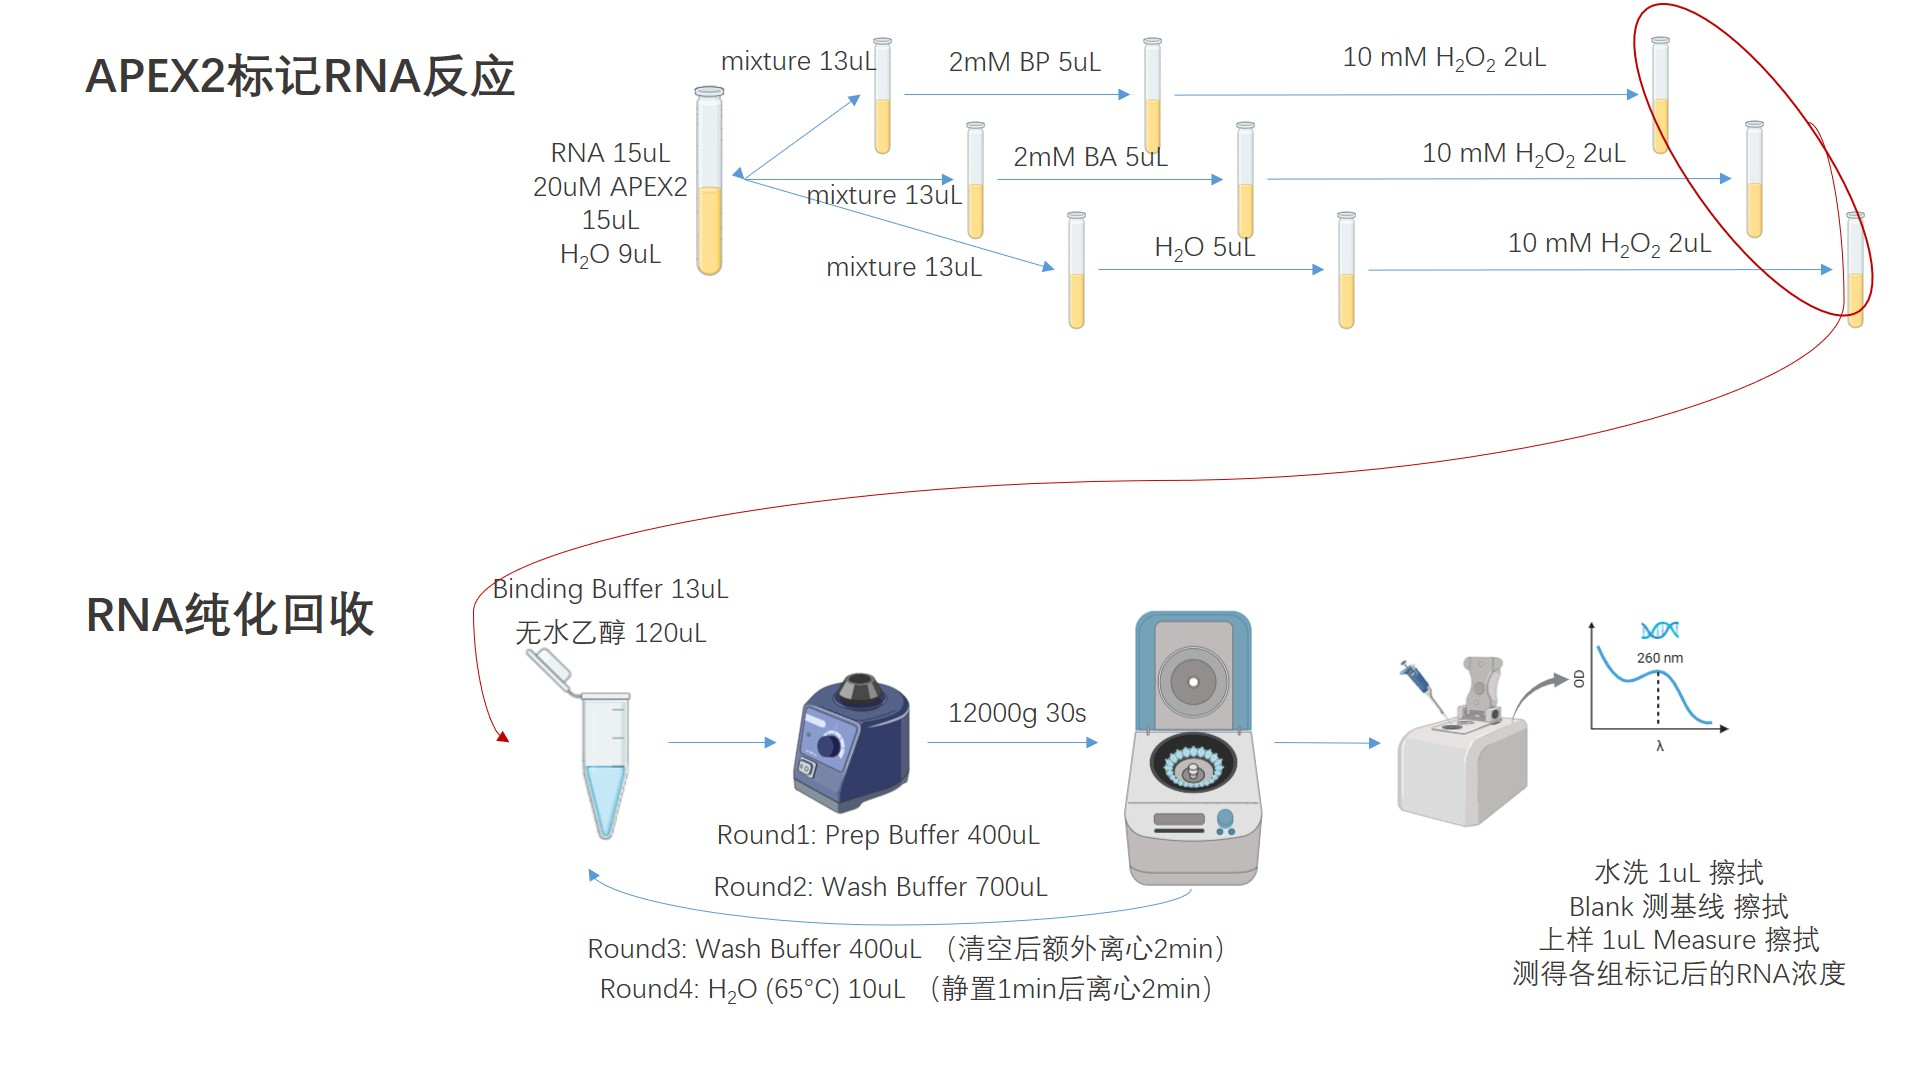
\includegraphics[width=1\linewidth]{../Figures/procedure1.jpg}}
    \subfigure{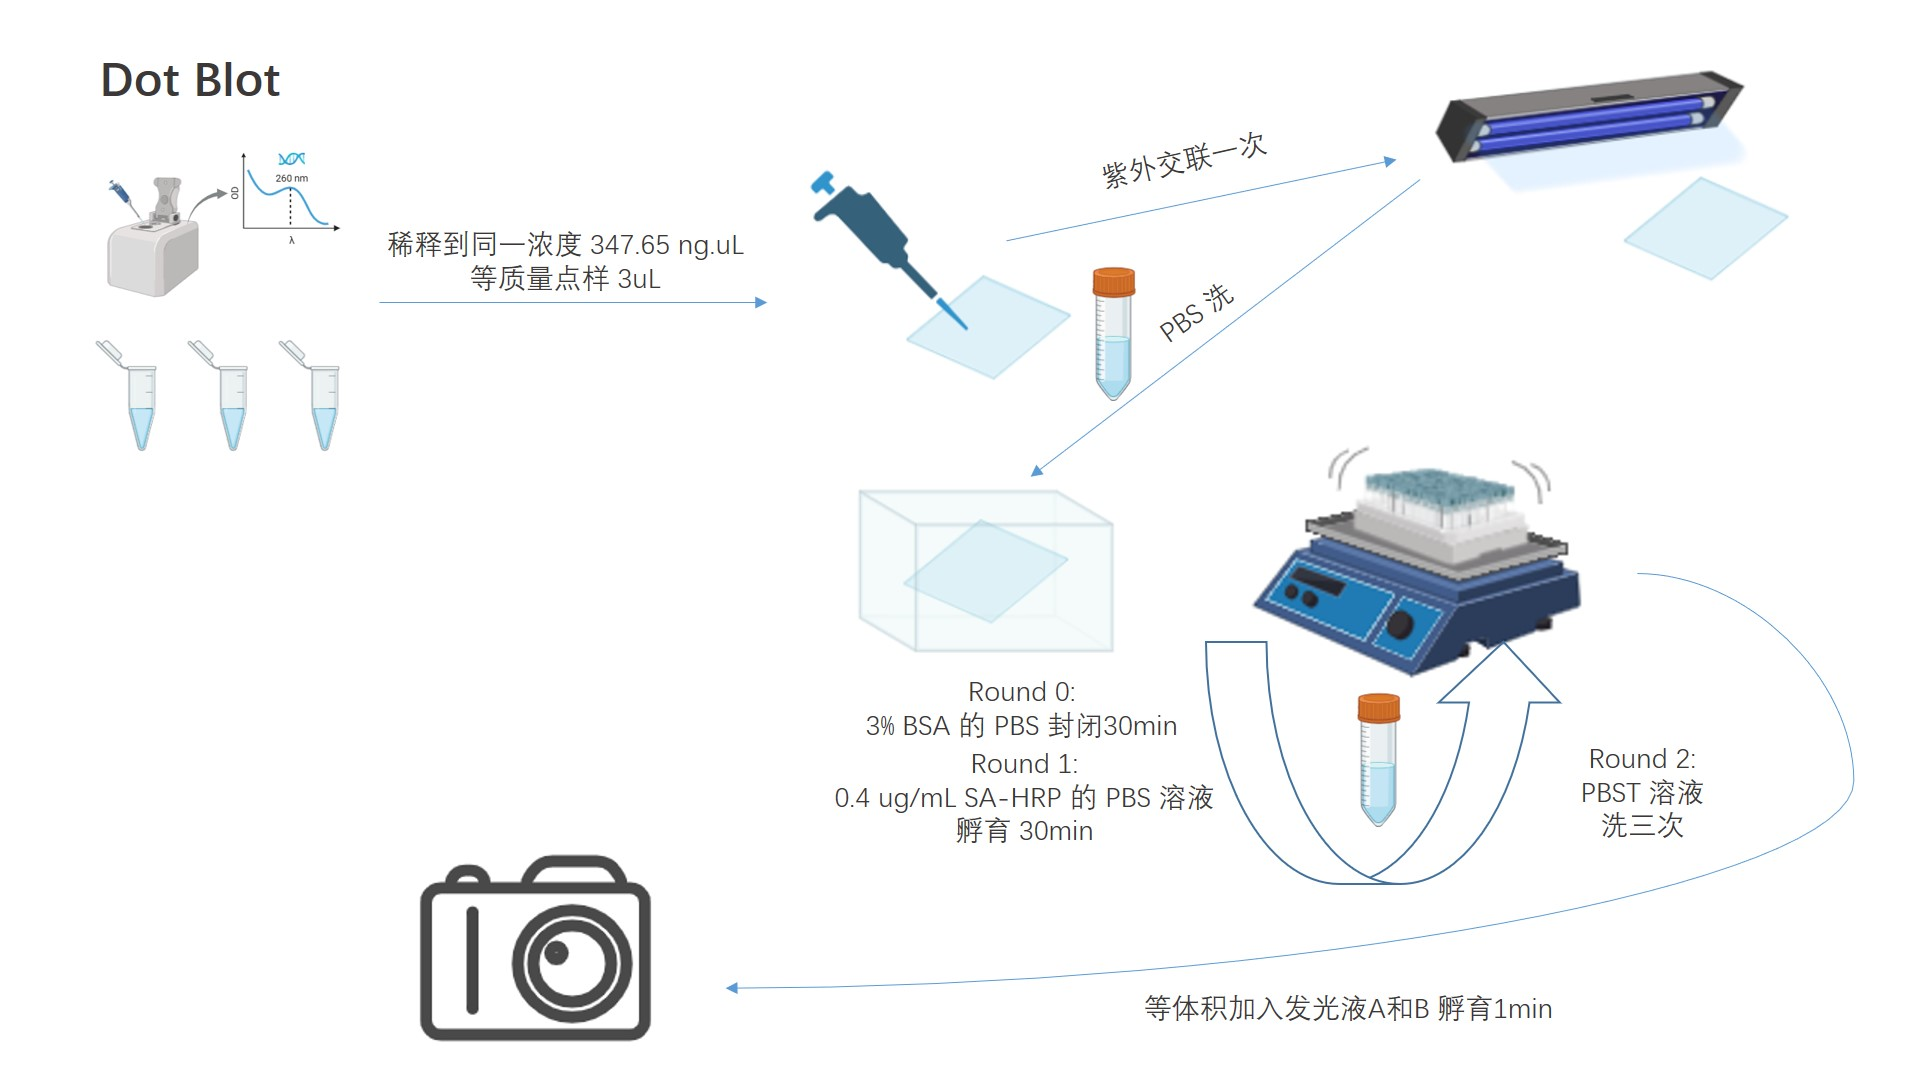
\includegraphics[width=1\linewidth]{../Figures/procedure2.jpg}}
    \caption{实验流程图}  
    \label{实验流程图}
 \end{figure}
 \begin{figure}
    \centering
    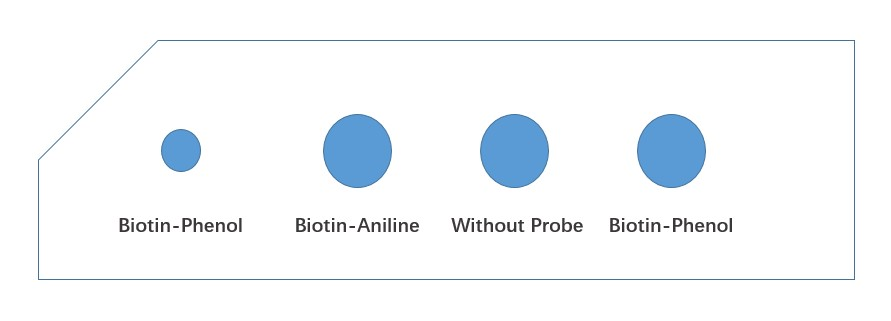
\includegraphics[width=0.7\linewidth]{../Figures/dotting.jpg}
    \caption{点样顺序与位置}
    \label{点样顺序与位置}
\end{figure}
\subsection{RNA纯化与浓度测定}
经过APEX2酶标记反应的RNA需要经过纯化之后再点样。
纯化的方式使用了商用试剂盒,大体上先将RNA吸附于柱子之上,然后用漂洗液洗去蛋白等杂质,最终用水洗脱。
后续的浓度测定使用NanoDrop 仪器,主要根据260nm处的吸光度换算而来。A260与A280的比值在1.8到2之间表面蛋白杂质较少。

\subsection{Dot Blot}
RNA的Dot Blot相当于Southern Blot的简化版本(核酸没有经过分离)。
首先是点样到Nylon膜上。由于RNA溶于高盐溶液,被点到Nylon膜上之后,并没有形成共价连接,并不稳定。
所以需要在UV紫外光下进行共价交联。

共价交联之后用PBS(Phosphate-Buffered Saline)清洗杂质蛋白,而后用含有BSA(Bovine Serum Albumin)的PBS溶液进行“封闭”(BSA作为阻断剂),这样可以用BSA蛋白覆盖住没有点样的区域,从而阻止杂质蛋白的结合。
经过封闭后,用含有SA-HRP蛋白的PBS溶液孵育随后用PBST(Phosphate-Buffered Saline with Tween-20)缓冲液清洗掉非特异性结合样品点的SA-HRP,这样可以使后续样品点可视化。
上述的PBST中含有的Tween-20是一种非离子型表面活性剂,降低表面张力有助于洗脱非特异性结合的蛋白。

\section{实验流程}
实验流程见图\ref{实验流程图}


其中点样的顺序与位置见图\ref{点样顺序与位置}。

\section{实验结果与分析}
经过ChemiDoc成像系统成像的结果见图\ref{实验结果}。
这个实验结果是极其出乎意料,因而发人深省的。

\begin{figure}[h]
    \centering
    \subfigure[第一轮成像]{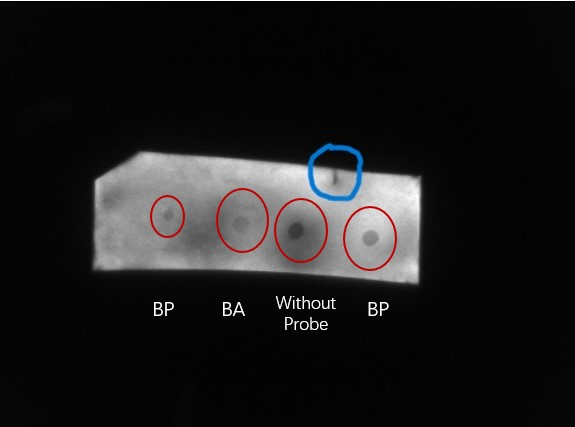
\includegraphics[width=0.3\linewidth]{../Figures/attempt1.jpg}}
    \subfigure[第二轮成像]{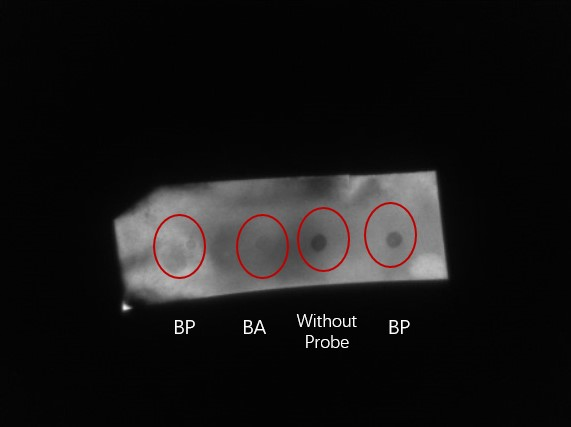
\includegraphics[width=0.3\linewidth]{../Figures/attempt2.jpg}}
    \subfigure[第三轮成像]{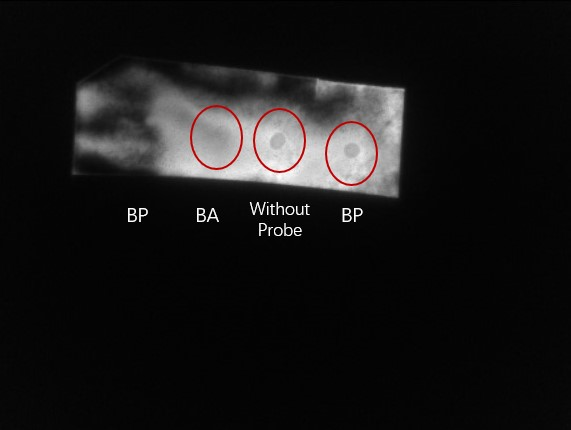
\includegraphics[width=0.3\linewidth]{../Figures/attempt3.jpg}}
    \caption{实验结果}  
    \label{实验结果}
 \end{figure}

上面是三次成像的结果,首先有一些现象是符合预期的:
\begin{itemize}
    \item Biotin-phenol和Biotin-aniline上样点呈现出了和背景不同的颜色
    \begin{itemize}
        \item 这说明探针有效的标记了RNA
    \end{itemize}
    \item Biotin-phenol标记的上样点,经过三轮漂洗成像后仍然比较清晰
    \item 然而Biotin-aniline标记的上样点,经过三轮漂洗后比较模糊
    \begin{itemize}
        \item 这说明Biotin-phenol特异性标记RNA的稳定性比较强
        \item 相较之下,在本次实验中,Biotin-aniline特异性标记RNA的稳定性要弱一些
    \end{itemize}
\end{itemize}

然而对比之下,体现出的反常之处如下:
\begin{itemize}
    \item 没有加探针的对照组颜色最深,呈现的标记效率竟然远远高于两个实验组。
    \item 没有上样的部分,成像黑白颜色不稳定。
    \item Biotin-aniline样点,经过反复清洗成像后,与周围环境界限不清。
    \item 人眼观测,未上样区域呈现淡黄色,而上样点为白色。
\end{itemize}


可能的原因和改进方向如下:
\begin{itemize}
    \item ChemiDoc成像系统成像结果的黑与白,受多种因素的影响。
    \begin{itemize}
        \item 比如图\ref{实验结果}中蓝色圆圈圈出的黑色竖线是由于物理上的裂口导致的,而不是有核酸或是蛋白。
        \item 发光液浸泡Nylon膜,置于空气中本身也会引起Nylon膜颜色变深。这是直接观察的结果。
        \item 反复的漂洗过程,进一步清除SA-HRP蛋白(主要清除非特异性结合的蛋白,但也削弱了特异性结合的蛋白)理论上也会引起颜色的改变。
        \item 所以对照组颜色深可能是因为点样时候枪头刮到Nylon膜导致的。
        \item 这一次对照组的结果大概率是干扰因素在其主导作用,应该废除重做。
    \end{itemize}
    \item 没有上样的部分,成像黑白颜色不稳定。
    \begin{itemize}
        \item 这可能由于防止Nylon膜时候产生的气泡导致
        \item 同时也注意到,多种颜色压缩成黑白两色,黑不一定是同一种黑,而可能是其它颜色的干扰。
    \end{itemize}
    \item 未上样区域可能受到环境污染
    \begin{itemize}
        \item 应该延长封闭时间,从30 min 延长到1 hour,进一步阻断杂质蛋白的非特异性结合。
        \item 紫外交联后的第一次清洗也可以使用含BSA的PBS溶液,这样可以进一步阻断杂质蛋白的结合。
    \end{itemize}
    \item 反复涂抹发光液可能引发其它问题,以后应该一次性清洗彻底后再涂发光液。
    \item 与此同时,有必要增设一些平行实验,用以排除干扰因素。
\end{itemize}
 




\bibliographystyle{plain}
\bibliography{references}
\end{document}